\section{Breitensuche}
%https://www.iro.umontreal.ca/~hahn/IFT3545/GTWA.pdf
\subsection{Einf\"uhrung}

\paragraph{Modellierung mit Graphen:} Wir haben gesehen dass ein Graph aus Knoten und Kanten besteht, wobei eine Kante jeweils zwei Knoten verbindet. Viele Probleme aus unserem Alltag k\"onnen mit diesen Grundelementen repr\"asentiert werden. Zum Beispiel kann man das Netz des \"offentlichen Verkehrs als Graphen darstellen, indem man alle Stationen als Knoten abbildet, und die Linien, die die Stationen verbinden, als gerichtete Kanten im Graphen, je nachdem in welche Richtung die Verkehrsmittel von der einen Station zur n\"achsten fahren k\"onnen.

\paragraph{Traversieren eines Graphen:}Es gibt viele verschiedene Algorithmen f\"ur Graphen, und eine wichtige Klasse von Algorithmen ist das Durchsuchen bzw. Traversieren von Graphen. Beim Traversieren eines Graphen werden die Knoten des Graphen besucht, und man bewegt sich dabei entlang den Kanten. Der Graph kann auch traversiert werden, um einen bestimmten Knoten im Graphen zu suchen.

\begin{figure}[htb]
\begin{center}
\begin{tikzpicture}[->,>=stealth',shorten >=1pt,auto,node distance=2cm,
                    semithick, style=circle]
  \tikzstyle{wstate}=[fill=white,text=black,draw=black]
  \tikzstyle{gstate}=[fill=gray,text=black,draw=black]
  \tikzstyle{bstate}=[fill=black,text=white,draw=black]
  
  \node[wstate] 		(0)                    {$0$};
  \node[wstate]         (1) [below left of=0] {$1$};
  \node[wstate]         (2) [below right of=1] {$2$};
  \node[wstate]         (3)  [right of=0] {$3$};
  \node[wstate]         (4) [ right of=2]       {$4$};
  \node[wstate]         (5) [above right of=4]    {$5$};

  \path (0) edge    [bend right]        node {} (1)
            	edge           node {} (3)
        (1) 	edge [bend right]	node {} (2)       
        (2) 	edge 	node {} (4)
        (3)	 edge    [bend left]          node {} (1)
        (4) 	edge node {} (3)
         (5) 	edge [bend left] node {} (4);

\end{tikzpicture}
\caption{Ein Beispiel-Graph}
\label{fig:bfs:graph}
\end{center}
\end{figure}

\paragraph{Erreichbarkeit:}Betrachten Sie den Graphen in Abb.~\ref{fig:bfs:graph}. Ausgehend von einem Startknoten m\"ochten wir untersuchen, ob ein Zielknoten erreichbar ist oder nicht. Ist der Knoten 2 von Knoten 0 aus erreichbar? Ist Knoten 5 auch erreichbar?

Um diese Fragen zu beantworten haben Sie vermutlich automatisch den Graphen betrachtet und visuell beurteilt, ob Sie vom Knoten 0 aus gewissen Kanten folgen k\"onnen um den Zielknoten zu erreichen.

\begin{figure}[htb]
\begin{center}
\begin{tikzpicture}[->,>=stealth',shorten >=1pt,auto,node distance=2.8cm,
                    semithick, style=circle]
  \tikzstyle{wstate}=[fill=white,text=black,draw=black,scale=0.7]
  \tikzstyle{gstate}=[fill=gray,text=black,draw=black]
  \tikzstyle{bstate}=[fill=black,text=white,draw=black]
  
  \node[wstate] 		(0)                    {$0$};
  \node[wstate]         (1) [above of=0] {$1$};
  \node[wstate]         (2) [above left of=0, node distance=2.3cm] {$2$};
  \node[wstate]         (3) [left of=0, node distance=3.5cm] {$3$};
  \node[wstate]         (4) [below left of=0] {$4$};
  \node[wstate]         (5) [below of=0, node distance=3.5cm] {$5$};
  \node[wstate]         (6) [below right of=0, node distance=3.4cm] {$6$};
  \node[wstate]         (7) [right of=0, node distance=5cm] {$7$};
  \node[wstate]         (8) [above right of=0] {$8$};
  \node[wstate]         (9) [above left of=3, node distance=2.2cm] {$9$};
  \node[wstate]         (10) [left of=3, node distance=2.5cm] {$10$};
  \node[wstate]         (11) [below left of=3, node distance=2.2cm] {$11$};
  \node[wstate]         (12) [above right of=8, node distance=2.2cm] {$12$};
  \node[wstate]         (13) [right of=8, node distance=2.5cm] {$13$};
  \node[wstate]         (14) [right of=6,node distance=2.2cm] {$14$};
  \node[wstate]         (15) [below right of=6, node distance=2.5cm] {$15$};
  \node[wstate]         (16) [below of=6, node distance=2.2cm] {$16$};

  \path (0) edge           node {} (1)
            	edge           node {} (2)
		edge           node {} (3)
		edge           node {} (4)
		edge           node {} (5)
		edge           node {} (6)
		edge           node {} (8)
	(1)	edge  [bend right]         node {} (3)
        (3)	edge           node {} (9)
	         edge          node {} (10)
	         edge          node {} (11)
        (4)	edge  [bend right]         node {} (13)
        (5)	edge  [bend left]         node {} (11)
       		 edge        node {} (6)
        (7) 	edge 	  node {} (0)
	        edge [bend left]	  node {} (6)
        (8) 	edge 	  node {} (12)
	        edge 	  node {} (13)
	        edge [bend left]	  node {} (5)
	 (9) 	edge [bend left]	  node {} (1)
         (6) 	edge 	  node {} (14)
         	edge 	  node {} (15)
	(11) 	edge 	  node {} (0)
		edge [bend right]	  node {} (16)
	(16) 	edge node {} (6)
         ;

\end{tikzpicture}
\caption{Ein etwas komplexerer Graph}
\label{fig:bfs:graph2}
\end{center}
\end{figure}

\paragraph{}Betrachten Sie nun den Graphen in Abb.\ref{fig:bfs:graph2} und beurteilen Sie, ob man von Knoten 7 den Knoten 16 erreichen kann. Kann man von Knoten 5 den Knoten 1 erreichen?

Wie Sie merken, ist das L\"osen der Aufgabe in einem etwas komplizierteren Graphen schon viel schwieriger. Stellen Sie sich jetzt aber vor, Sie haben einen Graphen mit tausenden von Knoten vor sich. Eine visuelle Beurteilung wird nun fast unm\"oglich und das Problem ist von Hand nicht mehr l\"osbar. Wir m\"ochten also einen Algorithmus entwickeln, damit ein Computer das Problem f\"ur uns l\"osen kann. Ein Computer kann aber nicht auf eine visuelle Beurteilung zur\"uckgreifen. Er braucht eine Repr\"asentation des Graphen, z.B. eine Adjazenzmatrix, mit welcher er arbeiten kann. Mit Hilfe der Adjazenzmatrix kann er dann jeweils f\"ur einen Knoten seine Nachbarsknoten ``sehen''. Um nun gewisse Probleme zu l\"osen braucht er zus\"atzlich zur Repr\"sentation als Adjazenzmatrix auch noch Instruktionen, die ihm mitteilen, wie das Problem \"uberhaupt gel\"ost werden kann.

\paragraph{Algorithmus entwickeln:}Wir m\"ochten also einen Algorithmus entwickeln, der f\"ur einen Startknoten $s$ in einem Graphen beurteilen kann, ob ein anderer Knoten von $s$ aus erreichbar ist oder nicht. Bei der Beantwortung der Frage zu den Graphen in Abb.~\ref{fig:bfs:graph} und ~\ref{fig:bfs:graph2} haben Sie wahrscheinlich intuitiv begonnen, ein paar Wege auszuprobieren und je nachdem wieder zu verwerfen, z.B. wenn Sie gemerkt haben, dass Sie von einem Knoten aus nicht mehr weiter kommen. Damit das Problem von einem Computer gel\"ost werden kann braucht er aber ein klares, strukturierteres Vorgehen, um die Frage nach der Erreichbarkeit zu beantworten.

Es gibt verschiedene Ans\"atze f\"ur ein solches Vorgehen. Bevor wir nun ein solches entwickeln \"uberlegen wir uns noch zus\"atzlich, ob wir ausser der Erreichbarkeit sonst noch Informationen haben wollen. Wenn wir herausgefunden haben, dass ein Knoten von einem Startknoten aus erreichbar ist, m\"ochten wir oftmals auch gerne wissen, wie weit entfernt er ist (in Anzahl Kanten, \"uber die der Knoten erreicht werden kann). Falls es mehrere Wege zum Knoten gibt sind wir h\"aufig an der k\"urzesten Distanz interessiert. Nicht zuletzt interessiert uns dann auch der konkrete Weg, der vom Startknoten zum Zielknoten f\"uhrt.

\paragraph{K\"urzester Weg:}Im Graphen aus Abb.~\ref{fig:bfs:graph} ist Knoten 4 von Knoten 0 \"uber Knoten 1 und 2 erreichbar (s.  Abb.~\ref{fig:bfs:graph:pathblue}), aber auch \"uber Knoten 3, 1, und 2 (s. Abb.~\ref{fig:bfs:graph:pathred}). Der erste Weg ist jedoch der K\"urzere: er traversiert nur 3 Kanten, w\"ahrend der zweite Weg 4 Kanten traversiert.

\begin{figure}[htb]
\begin{center}
\begin{tikzpicture}[->,>=stealth',shorten >=1pt,auto,node distance=2cm,
                    semithick, style=circle, scale=0.45]
  \tikzstyle{wstate}=[fill=white,text=black,draw=black]
  \tikzstyle{gstate}=[fill=gray,text=black,draw=black]
  \tikzstyle{bstate}=[fill=black,text=white,draw=black]
  
  \node[wstate] 		(0)                    {$0$};
  \node[wstate]         (1) [below left of=0] {$1$};
  \node[wstate]         (2) [below right of=1] {$2$};
  \node[wstate]         (3)  [right of=0] {$3$};
  \node[wstate]         (4) [ right of=2]       {$4$};
  \node[wstate]         (5) [above right of=4]    {$5$};

  \path (0) edge    [bend right,color=blue,very thick]        node {} (1)
            	edge           node {} (3)
        (1) 	edge [bend right, color=blue,very thick]	node {} (2)       
        (2) 	edge [color=blue,very thick]	node {} (4)
        (3)	 edge    [bend left]          node {} (1)
        (4) 	edge node {} (3)
         (5) 	edge [bend left] node {} (4);

\end{tikzpicture}
\caption{Weg von Knoten 0 zu Knoten 4 \"uber Knoten 1 und 2}
\label{fig:bfs:graph:pathblue}
\end{center}
\end{figure}

\begin{figure}[htb]
\begin{center}
\begin{tikzpicture}[->,>=stealth',shorten >=1pt,auto,node distance=2cm,
                    semithick, style=circle, scale = 0.45]
  \tikzstyle{wstate}=[fill=white,text=black,draw=black]
  \tikzstyle{gstate}=[fill=gray,text=black,draw=black]
  \tikzstyle{bstate}=[fill=black,text=white,draw=black]
  
  \node[wstate] 		(0)                    {$0$};
  \node[wstate]         (1) [below left of=0] {$1$};
  \node[wstate]         (2) [below right of=1] {$2$};
  \node[wstate]         (3)  [right of=0] {$3$};
  \node[wstate]         (4) [ right of=2]       {$4$};
  \node[wstate]         (5) [above right of=4]    {$5$};

  \path (0) edge    [bend right]        node {} (1)
            	edge    [color=red,very thick]       node {} (3)
        (1) 	edge [bend right, color=red,very thick]	node {} (2)       
        (2) 	edge [color=red,very thick]	node {} (4)
        (3)	 edge    [bend left, color=red,very thick]          node {} (1)
        (4) 	edge node {} (3)
         (5) 	edge [bend left] node {} (4);

\end{tikzpicture}
\caption{Weg von Knoten 0 zu Knoten 4 \"uber Knoten 3, 1 und 2}
\label{fig:bfs:graph:pathred}
\end{center}
\end{figure}



\begin{aufg}
Wir m\"ochten nun also ein Vorgehen entwickeln, welches in einem Graphen von einem Startknoten aus einen Knoten auf dem k\"urzesten Weg sucht und uns dar\"uber informiert, ob er vom Startknoten aus erreichbar ist. \"Uberlegen Sie sich, wie so ein Vorgehen aussehen k\"onnte.
\end{aufg}

\subsection{Algorithmus}\label{subsec:algorithm}

Wie wir schon erw\"ahnt haben gibt es mehrere M\"oglichkeiten f\"ur ein Vorgehen, welches einen Graphen traversiert und nach einem bestimmten Knoten sucht. In diesem Kapitel werden wir einen Algorithmus,  n\"amlich die Breitensuche, Schritt f\"ur Schritt erarbeiten. Die Breitensuche erm\"oglicht es uns n\"amlich einen Knoten zu suchen, und, falls er gefunden wurde, seine k\"urzeste Distanz beziehungsweise auch den konkreten Weg zum Knoten ganz einfach herauszufinden.

Der Algorithmus f\"ur die Breitensuche ben\"otigt drei Inputs: einen Graphen, einen Startknoten und einen Zielknoten. In einem ersten Schritt wird der Startknoten betrachtet. Im Graphen in  Abb.~\ref{fig:bfs:bfs1} k\"onnen vom Startknoten 0 aus alle seine Nachbarn, n\"amlich die Knoten 1 und 3 erreicht werden. Alle Nachbarn, die von diesem Startknoten aus erreichbar sind, werden grau eingef\"arbt.

\begin{figure}[htb]
\begin{center}
\begin{tikzpicture}[->,>=stealth',shorten >=1pt,auto,node distance=2cm,
                    semithick, style=circle]
  \tikzstyle{rstate}=[fill=white!80!red,text=red,draw=red]
  \tikzstyle{wstate}=[fill=white,text=black,draw=black]
  \tikzstyle{gstate}=[fill=gray!30!white,text=black,draw=black]
  \tikzstyle{bstate}=[fill=black,text=white,draw=black]
  
  \node[rstate] 		(0)                  {$0$};
  \node[gstate]         (1) [below left of=0] {$1$};
  \node[wstate]         (2) [below right of=1] {$2$};
  \node[gstate]         (3)  [right of=0] {$3$};
  \node[wstate]         (4) [ right of=2]       {$4$};
  \node[wstate]         (5) [above right of=4]    {$5$};

  \path (0) edge    [bend right]        node {} (1)
            	edge           node {} (3)
        (1) 	edge [bend right]	node {} (2)       
        (2) 	edge 	node {} (4)
        (3)	 edge    [bend left]          node {} (1)
        (4) 	edge node {} (3)
         (5) 	edge [bend left] node {} (4);

\end{tikzpicture}
\caption{Startknoten (rot) und seine Nachbarn (grau)}
\label{fig:bfs:bfs1}
\end{center}
\end{figure}


Wir m\"ochten nun zum Beispiel wissen, ob Knoten 2 von diesem Startknoten aus erreichbar ist. Als Erstes pr\"ufen wir also, ob sich der Knoten unter den Nachbarn des Startknotens befindet. Da dies nicht der Fall ist, m\"ussen wir weitersuchen. Da wir mit Distanz 1 den Knoten nicht gefunden haben, m\"ussen wir bei einer gr\"osseren Distanz weitersuchen, also betrachten wir alle Knoten, die mit einer maximalen Distanz von 2 vom Startknoten aus erreichbar sind. Dies sind alle Knoten, die von den Nachbarn des Startknotens aus erreichbar sind. Wir w\"ahlen also zuerst den ersten Nachbarn, Knoten 1, und betrachten dessen Nachbarn. 

\begin{figure}[htb]
\begin{center}
\begin{tikzpicture}[->,>=stealth',shorten >=1pt,auto,node distance=2cm,
                    semithick, style=circle, scale=0.45]
  \tikzstyle{rstate}=[fill=white!80!red,text=red,draw=red]
  \tikzstyle{wstate}=[fill=white,text=black,draw=black]
  \tikzstyle{gstate}=[fill=gray!30!white,text=black,draw=black]
  \tikzstyle{bstate}=[fill=black,text=white,draw=black]
  
  \node[wstate] 		(0)                  {$0$};
  \node[rstate]         (1) [below left of=0] {$1$};
  \node[gstate]         (2) [below right of=1] {$2$};
  \node[wstate]         (3)  [right of=0] {$3$};
  \node[wstate]         (4) [ right of=2]       {$4$};
  \node[wstate]         (5) [above right of=4]    {$5$};

  \path (0) edge    [bend right]        node {} (1)
            	edge           node {} (3)
        (1) 	edge [bend right]	node {} (2)       
        (2) 	edge 	node {} (4)
        (3)	 edge    [bend left]          node {} (1)
        (4) 	edge node {} (3)
         (5) 	edge [bend left] node {} (4);

\end{tikzpicture}
\qquad
\begin{tikzpicture}[->,>=stealth',shorten >=1pt,auto,node distance=2cm,
                    semithick, style=circle,scale=0.45]
  \tikzstyle{rstate}=[fill=white!80!red,text=red,draw=red]
  \tikzstyle{wstate}=[fill=white,text=black,draw=black]
  \tikzstyle{gstate}=[fill=gray!30!white,text=black,draw=black]
  \tikzstyle{bstate}=[fill=black,text=white,draw=black]
  
  \node[wstate] 		(0)                  {$0$};
  \node[gstate]         (1) [below left of=0] {$1$};
  \node[wstate]         (2) [below right of=1] {$2$};
  \node[rstate]         (3)  [right of=0] {$3$};
  \node[wstate]         (4) [ right of=2]       {$4$};
  \node[wstate]         (5) [above right of=4]    {$5$};

  \path (0) edge    [bend right]        node {} (1)
            	edge           node {} (3)
        (1) 	edge [bend right]	node {} (2)       
        (2) 	edge 	node {} (4)
        (3)	 edge    [bend left]          node {} (1)
        (4) 	edge node {} (3)
         (5) 	edge [bend left] node {} (4);

\end{tikzpicture}
\caption{Aktuell betrachtete Knoten (rot) und ihre Nachbarn (grau)}
\label{fig:bfs:bfs2}
\end{center}
\end{figure}

In Abb.~\ref{fig:bfs:bfs2} sehen wir, dass der Knoten 2 der einzige Nachbarknoten von Knoten 1 ist. Nun betrachten wir auch noch den 2. Nachbarn unseres Startknotens, n\"amlich Knoten 3, und betrachten dessen Nachbarn. Der einzige Nachbarknoten von Knoten 3 ist Knoten 1, welchen wir aber gerade eben schon betrachtet haben und deshalb nicht mehr betrachten m\"ussen. Wir m\"ussen uns also irgendwie merken, welche Knoten wir schon betrachtet haben, damit wir sie nicht nochmals bearbeiten wenn wir sp\"ater auf einem anderen Weg nochmals darauf stossen. 

Wir erreichen dies, indem wir einen betrachteten Knoten speziell markieren, beispielsweise indem wir ihn schwarz einf\"arben. Gleichzeitig f\"arben wir Knoten, die wir als Nachbarn eines Knoten schon entdeckt haben, aber noch nicht bearbeiten haben, grau ein. Abb.~\ref{fig:bfs:bfs3} zeigt den Graphen, nachdem der Startknoten (Knoten 0) betrachtet wurde (links), nachdem sein erster Nachbar (Knoten 1) betrachtet wurde (Mitte) und nachdem sein zweiter Nachbar (Knoten 3) betrachtet wurde (rechts).

\begin{figure}[htb]
\begin{center}
\begin{tikzpicture}[->,>=stealth',shorten >=1pt,auto,node distance=1.5cm,
                    semithick, style=circle, scale=0.2]
  \tikzstyle{rstate}=[fill=white!80!red,text=red,draw=red]
  \tikzstyle{wstate}=[fill=white,text=black,draw=black]
  \tikzstyle{gstate}=[fill=gray!30!white,text=black,draw=black]
  \tikzstyle{bstate}=[fill=black,text=white,draw=black]
  
  \node[bstate] 		(0)                  {$0$};
  \node[gstate]         (1) [below left of=0] {$1$};
  \node[wstate]         (2) [below right of=1] {$2$};
  \node[gstate]         (3)  [right of=0] {$3$};
  \node[wstate]         (4) [ right of=2]       {$4$};
  \node[wstate]         (5) [above right of=4]    {$5$};

  \path (0) edge    [bend right]        node {} (1)
            	edge           node {} (3)
        (1) 	edge [bend right]	node {} (2)       
        (2) 	edge 	node {} (4)
        (3)	 edge    [bend left]          node {} (1)
        (4) 	edge node {} (3)
         (5) 	edge [bend left] node {} (4);

\end{tikzpicture}
\qquad
\begin{tikzpicture}[->,>=stealth',shorten >=1pt,auto,node distance=1.5cm,
                    semithick, style=circle,scale=0.2]
  \tikzstyle{rstate}=[fill=white!80!red,text=red,draw=red]
  \tikzstyle{wstate}=[fill=white,text=black,draw=black]
  \tikzstyle{gstate}=[fill=gray!30!white,text=black,draw=black]
  \tikzstyle{bstate}=[fill=black,text=white,draw=black]
  
  \node[bstate] 		(0)                  {$0$};
  \node[bstate]         (1) [below left of=0] {$1$};
  \node[gstate]         (2) [below right of=1] {$2$};
  \node[gstate]         (3)  [right of=0] {$3$};
  \node[wstate]         (4) [ right of=2]       {$4$};
  \node[wstate]         (5) [above right of=4]    {$5$};

  \path (0) edge    [bend right]        node {} (1)
            	edge           node {} (3)
        (1) 	edge [bend right]	node {} (2)       
        (2) 	edge 	node {} (4)
        (3)	 edge    [bend left]          node {} (1)
        (4) 	edge node {} (3)
         (5) 	edge [bend left] node {} (4);

\end{tikzpicture}
\qquad
\begin{tikzpicture}[->,>=stealth',shorten >=1pt,auto,node distance=1.5cm,
                    semithick, style=circle,scale=0.2]
  \tikzstyle{rstate}=[fill=white!80!red,text=red,draw=red]
  \tikzstyle{wstate}=[fill=white,text=black,draw=black]
  \tikzstyle{gstate}=[fill=gray!30!white,text=black,draw=black]
  \tikzstyle{bstate}=[fill=black,text=white,draw=black]
  
  \node[bstate] 		(0)                  {$0$};
  \node[bstate]         (1) [below left of=0] {$1$};
  \node[gstate]         (2) [below right of=1] {$2$};
  \node[bstate]         (3)  [right of=0] {$3$};
  \node[wstate]         (4) [ right of=2]       {$4$};
  \node[wstate]         (5) [above right of=4]    {$5$};

  \path (0) edge    [bend right]        node {} (1)
            	edge           node {} (3)
        (1) 	edge [bend right]	node {} (2)       
        (2) 	edge 	node {} (4)
        (3)	 edge    [bend left]          node {} (1)
        (4) 	edge node {} (3)
         (5) 	edge [bend left] node {} (4);

\end{tikzpicture}

\caption{Verlauf der Einf\"arbungen}
\label{fig:bfs:bfs3}
\end{center}
\end{figure}

Im n\"achsten Durchlauf wird der n\"achste graue Knoten, also Knoten 2, betrachtet. Knoten 2 war der gesuchte Knoten - das heisst wir haben den Knoten gefunden!

\begin{figure}[htb]
\begin{center}
\begin{tikzpicture}[->,>=stealth',shorten >=1pt,auto,node distance=2cm,
                    semithick, style=circle]
  \tikzstyle{zstate}=[fill=gray!30!white,text=black,draw=white!40!green,thick]
  \tikzstyle{wstate}=[fill=white,text=black,draw=black]
  \tikzstyle{gstate}=[fill=gray!30!white,text=black,draw=black]
  \tikzstyle{bstate}=[fill=black,text=white,draw=black]
  
  \node[bstate] 		(0)                  {$0$};
  \node[bstate]         (1) [below left of=0] {$1$};
  \node[zstate]         (2) [below right of=1] {$2$};
  \node[bstate]         (3)  [right of=0] {$3$};
  \node[wstate]         (4) [ right of=2]       {$4$};
  \node[wstate]         (5) [above right of=4]    {$5$};

  \path (0) edge    [bend right]        node {} (1)
            	edge           node {} (3)
        (1) 	edge [bend right]	node {} (2)       
        (2) 	edge 	node {} (4)
        (3)	 edge    [bend left]          node {} (1)
        (4) 	edge node {} (3)
         (5) 	edge [bend left] node {} (4);

\end{tikzpicture}
\caption{Zielknoten (gr\"un markiert) wurde gefunden}
\label{fig:bfs:bfs4}
\end{center}
\end{figure}


\paragraph{Zusammenfassung:}Wir m\"ochten nun das Vorgehen zusammenfassen und in einem Algorithmus formulieren.

Wir beginnen mit einem Startknoten und f\"arben ihn sogleich grau ein. Der n\"achste zu betrachtende Knoten ist jeweils der n\"achste graue Knoten. Da anfangs nur den Startknoten grau ist, beginnen wir gleich mit diesem Knoten. Falls der Knoten der gesuchte Knoten ist, haben wir ihn gefunden und k\"onnen das Programm beenden. Andernfalls f\"arben wir alle Nachbarn des Knotens grau ein. Den betrachteten Knoten selbst f\"arben wir schwarz ein, um zu markieren, dass wir diesen nun bearbeitet haben. Wir fahren fort mit dem grauen Knoten, der als erstes grau gef\"arbt wurde und wiederholen das beschriebene Vorgehen. 

Es ist wichtig, dass die grauen Knoten in der Reihenfolge betrachtet werden, in der sie eingef\"arbt werden. Damit stellen wir sicher, dass zuerst alle Knoten von einer kleineren Distanz zum Startknoten bearbeitet werden als die weiter entfernten, da jene auch erst sp\"ater eingef\"arbt wurden. Man kann sich dies also wie eine Warteschlange vorstellen, in der die grauen Knoten eingereiht werden:  die Knoten die zuerst eingereiht wurden, werden auch zuerst wieder von der Warteschlage entfernt.

Dieses Vorgehen f\"uhrt uns nun zur Formulierung des Algorithmus f\"ur die Breitensuche.

\begin{algorithm}
\caption{Breitensuche}\label{alg:bfs}
\begin{algorithmic}[1]
\Procedure{Breitensuche}{$graph,start,ziel$}
	\State $start$ grau einf\"arben
   \State $graue Knoten = \lbrack start\rbrack$\Comment{Warteschlange f\"ur graue Knoten}
      \While{$graueKnoten \neq \emptyset$ }
   	\State $current \gets$ vorderster Knoten aus $graueKnoten$
	\If {$current = ziel$} 
   		\Return true\Comment{Zielknoten gefunden}
   	\EndIf
	\ForAll {$narchbar$ in \Call{nachbarknoten}{$graph, current$}}\label{alg:bfs:line:nachbarn}
		\If {$nachbar$ nicht schwarz und nicht grau}\Comment{Neu entdeckter Knoten}
		 	\State $nachbar$ grau einf\"arben
			\State $nachbar$ zuhinterst in $graueKnoten$ einreihen
		\EndIf
	\EndFor
	\State $current$ schwarz einf\"arben\Comment{Knoten fertig bearbeitet}
	\State $current$ aus $graueKnoten$ entfernen
   \EndWhile\label{euclidendwhile}
   \State \textbf{return} false\Comment{Zielknoten nicht gefunden}
\EndProcedure
\end{algorithmic}
\end{algorithm}

\begin{aufg}
Benutzen Sie ihre Funktion \textsc{Nachbarknoten}, welche Sie bereits im vorhergehenden Kapitel geschrieben haben, um Algorithmus~\ref{alg:bfs} zu implementieren. Testen Sie Ihr Programm indem sie die Breitensuche f\"ur verschiedene Start- und Endknoten aufrufen.

\textbf{Hinweis:} Sie k\"onnen das Einf\"arben der Knoten so umsetzen, dass sie in einer Liste f\"ur jeden Knoten seine Farbe speichern. F\"ur die Umsetzung der Warteschlange der grauen Knoten k\"onnen Sie auch ein Array verwenden. Mit dem Befehl $pop(x)$ kann ein Element an Stelle x im Array ausgelesen und entfernt werden.
\end{aufg}

\subsection{Anwendung und Erweiterung}

Wir werden nun den entwickelten Algorithmus anhand eines konkreten Beispiels betrachten und weiterentwickeln.
%Zonen bei �V
%Stationen mit �V
%Soziale Netzwerke
%Computernetzwerke

\paragraph{Soziale Netzwerke:}In der heutigen Gesellschaft sind soziale Netzwerke zu einem wichtigen Werkzeug geworden, um Beziehungen zu pflegen, z.B. \"uber Berufsnetzwerke oder Freundesnetzwerke. Solche Netzwerke k\"onnen wir als Graphen modellieren. Mit Hilfe von Graphenalgorithmen k\"onnen gewisse Eigenschaften und Strukturen der Netzwerke erforscht werden.

In Abb.~\ref{bfs:ex:network} sehen Sie einige Personen und ihre Vernetzungen zu anderen Personen. Wir m\"ochten dieses kleine Personennetzwerk etwas genauer untersuchen, z.B. um herauszufinden, ob bestimmte Personen (auch \"uber andere Personen) miteinander vernetzt sind.

\begin{figure}[h]
\small
\begin{minipage}{0.15\linewidth}

\includegraphics[width=.9\textwidth]{../fig/profile.jpg}

Tom
\end{minipage} 
\begin{minipage}{0.15\linewidth}
  \textbf{Freunde}:\\
  Karin\\
  Tina
\end{minipage}
\begin{minipage}{0.15\linewidth}

\includegraphics[width=.9\textwidth]{../fig/profile.jpg}

John
\end{minipage}
\begin{minipage}{0.15\linewidth}
  \textbf{Freunde}:\\
  Tina\\
  Karin
\end{minipage}
\begin{minipage}{0.15\linewidth}

\includegraphics[width=.9\textwidth]{../fig/profile.jpg}

Jimmy
\end{minipage}
\begin{minipage}{0.15\linewidth}  
  \textbf{Freunde}:\\
  Lars\\
  Laura
\end{minipage}\par
\vspace{20pt}
\begin{minipage}{0.15\linewidth}

\includegraphics[width=.9\textwidth]{../fig/profile.jpg}

Karin
\end{minipage} 
\begin{minipage}{0.15\linewidth}
  \textbf{Freunde}:\\
  Tom\\
  Tina\\
  John
\end{minipage}
\begin{minipage}{0.15\linewidth}

\includegraphics[width=.9\textwidth]{../fig/profile.jpg}

Tina
\end{minipage}
\begin{minipage}{0.15\linewidth}
  \textbf{Freunde}:\\
  John\\
  Lars\\
  Anna\\
  Laura\\
  Karin\\
  Tom
\end{minipage}
\begin{minipage}{0.15\linewidth}

\includegraphics[width=.9\textwidth]{../fig/profile.jpg}
Lars
\end{minipage}
\begin{minipage}{0.15\linewidth}
  \textbf{Freunde}:\\
  Jimmy\\
  Laura\\
  Tina
\end{minipage}\par
\vspace{20pt}
\begin{minipage}{0.15\linewidth}

\includegraphics[width=.9\textwidth]{../fig/profile.jpg}

Anna
\end{minipage} 
\begin{minipage}{0.15\linewidth}
  \textbf{Freunde}:\\
  Tina\\
  Simon  
\end{minipage}
\begin{minipage}{0.15\linewidth}

\includegraphics[width=.9\textwidth]{../fig/profile.jpg}

Simon
\end{minipage}
\begin{minipage}{0.15\linewidth}
  \textbf{Freunde}:\\
  Anna\\
  Lars
\end{minipage}
\begin{minipage}{0.15\linewidth}

\includegraphics[width=.9\textwidth]{../fig/profile.jpg}

Laura
\end{minipage}
\begin{minipage}{0.15\linewidth}
  \textbf{Freunde}:\\
  Tina\\
  Lars\\
  Jimmy
\end{minipage}\\
\caption{Ein kleines Personennetzwerk}
\label{bfs:ex:network}
\end{figure}

Dieses Netzwerk kann mit einem ungerichteten Graphen modelliert werden, bei dem die Knoten die Personen repr\"asentieren und die Kanten die Freundschaftsbeziehungen zwischen den Personen. Den daraus resultierenden Graphen sehen Sie in Abb.~\ref{bfs:ex:networkgraph}

\begin{figure}[htb]
\begin{center}
\begin{tikzpicture}[-,>=stealth',shorten >=1pt,auto,node distance=4cm,
                    semithick, minimum size = 2em]
                    \usetikzlibrary{shapes}
    \tikzstyle{every node}=[ellipse, minimum width=60pt,
    align=center]
  \tikzstyle{zstate}=[fill=white!80!green,text=black!40!green,draw=black!40!green]
  \tikzstyle{wstate}=[fill=white,text=black,draw=black]
  \tikzstyle{gstate}=[fill=gray!30!white,text=black,draw=black]
  \tikzstyle{bstate}=[fill=black,text=white,draw=black]
  
  \node[wstate] 		(0)                  {Tom};
  \node[wstate]         (1) [right of=0] {John};
  \node[wstate]         (2) [right of=1] {Jimmy};
  \node[wstate]         (3)  [below of=0, node distance=2.5cm] {Karin};
  \node[wstate]         (4) [right of=3]       {Tina};
  \node[wstate]         (5) [right of=4]    {Lars};
  \node[wstate]         (6) [below of=3, node distance=2.5cm]    {Anna};
  \node[wstate]         (7) [right of=6]    {Simon};
  \node[wstate]         (8) [right of=7]    {Laura};

\draw (0)--(3)
	(0)--(4)
	(1)--(3)
	(1)--(4)
	(2)--(5)
	(3)--(4)
	(4)--(5)
	(4)--(6)
	(4)--(8)
	(5)--(7)
	(5)--(8)
	(6)--(7);
	
	\path  (2) edge    [bend left=70]        node {} (8);

\end{tikzpicture}
\caption{Modellierung des Personennetzwerks als Graph}
\label{bfs:ex:networkgraph}
\end{center}
\end{figure}

\begin{aufg}
Modellieren Sie diesen Graphen als Adjazenzmatrix und lesen Sie ihn in ihr bisheriges Programm ein. Benutzen Sie daf\"ur folgende Reihenfolge: Tom f\"ur Zeile/Spalte 0, John f\"ur Zeile/Spalte 1 und so weiter.
\end{aufg}

\begin{aufg}
Testen Sie mit ihrem Programm, ob es irgendeine Verbindung zwischen Anna und John gibt.
\end{aufg}

\begin{aufg}
Tina \"uberlegt sich schon seit einiger Zeit, das Netzwerk wieder zu verlassen. Falls sie tats\"achlich das Netzwerk verlassen w\"urde, g\"abe es dann trotzdem noch eine Verbindung von Anna zu Jimmy? Und von Simon zu Tom?
\end{aufg}

Wir k\"onnen mit unserem Programm jetzt also einfach beurteilen, ob es eine Verbindung zwischen zwei Personen gibt. Nun m\"ochten wir aber gerne wissen, \"uber wieviele Personen zwei Personen sozusagen miteinander verbunden sind. Wir m\"ussen also unseren Algorithmus so anpassen, dass wir am Ende sagen k\"onnen, wieviele Verbindungen eine Person von einer anderen Person mindestens entfernt ist. Beispiel: Wenn Anna mit Tina befreundet ist und Tina mit Lars, dann ist Lars \"uber zwei Freundschaftsbeziehungen mit Anna verbunden.

\begin{aufg}
\"Uberlegen Sie sich, wie der Algorithmus~\ref{alg:bfs} angepasst werden k\"onnte, sodass die Distanz zum Zielknoten gespeichert wird.
\textbf{Hinweis:} Es reicht nicht, die Distanz in einer einzigen Variablen zu Speichern. Wieso nicht?
\end{aufg}

Wenn wir beim Startknoten starten, dann sind alle seine Nachbarn mit einer Distanz von 1 erreichbar. Da wir bei der Breitensuche immer zuerst alle Knoten einer gewissen Distanz abarbeiten, bevor wir die Distanz erh\"ohen, wissen wir, dass wenn wir einen Knoten neu entdecken, dass dieser nicht \"uber irgendeinen Weg schneller erreichbar ist als \"uber den Knoten, von dem aus wir ihn entdeckt haben. Das heisst also, ein Knoten kann mit einer Distanz vom Vorg\"angerknoten + 1 erreicht werden. Da wir in unserem Algorithmus beim Abarbeiten der grauen Knoten nicht mehr wissen, wie weit diese vom Startknoten entfernt sind, k\"onnen wir nicht einfach in einer Variable die Distanz festhalten, auf der wir gerade suchen. Wir k\"onnen aber zu jedem neu entdeckten Knoten seine Distanz speichern, damit wir beim Bearbeiten des Knotens wissen, wie weit entfernt vom Startknoten wir uns befinden. Wenn wir schlussendlich den Zielknoten erreichen, k\"onnen wir ganz einfach seine Distanz auslesen. In Algorithmus~\ref{alg:bfs:distance} sehen Sie den Algorithmus mit der Erweiterung mit der Speicherung der Distanzen (rot markiert).

\begin{algorithm}
\caption{Breitensuche}\label{alg:bfs:distance}
\begin{algorithmic}[1]
\Procedure{Breitensuche}{$graph,start,ziel$}
	\State $start$ grau einf\"arben
   	\State $graue Knoten \gets \lbrack start\rbrack$\Comment{Warteschlange f\"ur graue Knoten}
	\textcolor{red}{\State $distanzen$ = array\lbrack Anzahl Knoten\rbrack}
      \While{$graueKnoten \neq \emptyset$ }
   	\State $current \gets$ vorderster Knoten aus $graueKnoten$
	\If {$current = ziel$} 
   		\Return true\Comment{Zielknoten gefunden}
   	\EndIf
	\ForAll {$narchbar$ in \Call{nachbarknoten}{$graph, current$}}\label{alg:bfs:line:nachbarn}
		\If {$nachbar$ nicht schwarz und nicht grau}\Comment{Neu entdeckter Knoten}
		 	\State $nachbar$ grau einf\"arben
			\State $nachbar$ zuhinterst in $graueKnoten$ einreihen
			\textcolor{red}{\State $distanzen\lbrack nachbar\rbrack = distanzen\lbrack current \rbrack + 1$}
		\EndIf
	\EndFor
	\State $current$ schwarz einf\"arben\Comment{Knoten fertig bearbeitet}
	\State $current$ aus $graueKnoten$ entfernen
   \EndWhile\label{euclidendwhile}
   \State \textbf{return} false\Comment{Zielknoten nicht gefunden}
\EndProcedure
\end{algorithmic}
\end{algorithm}


\begin{aufg}
Erg\"anzen Sie Ihr Programm so, dass am Schluss die k\"urzeste Distanz von einem Startknoten zu einem Zielknoten ausgelesen werden kann, falls der Zielknoten vom Startknoten aus erreichbar ist.
\end{aufg}

Wir haben nun also ein Programm, das uns sagen kann, wie weit entfernt ein Startknoten von einem Zielknoten mindestens liegt (falls der Zielknoten \"uberhaupt vom Startknoten aus erreichbar ist). Wir m\"ochten unseren Algorithmus nun noch etwas weiter ausbauen, so dass wir am Schluss, falls wir den Zielknoten gefunden haben, herausfinden k\"onnen, \"uber welche Knoten der k\"urzeste Weg vom Startknoten zum Zielknoten f\"uhrt. Wir m\"ussen uns also w\"ahrend dem Traversieren irgendwie merken, wie wir zu einem aktuellen Knoten gelangt sind. Es ist m\"oglich, dass es mehrere Wege von einem Startknoten zu einem Zielknoten gibt, aber wir sind stets am k\"urzesten Weg interessiert. Das heisst, wir k\"onnen w\"ahrend der Suche, beim Abarbeiten eines Knotens, einfach speichern, von welchem Knoten aus wir zu diesem Knoten gelangt sind. Dann k\"onnen wir vom Schlussknoten aus Knoten f\"ur Knoten zur\"uckverfolgen, auf welchem Weg wir zum Ziel gelangt sind.

\begin{mbsp}
In unserem Netzwerk aus Abb.~\ref{bfs:ex:network} ist Tom mit Karin befreundet und Karin mit John. Tom ist also \"uber Karin mit John verbunden. Ein m\"oglicher Pfad w\"are also Tom - Karin - John. Einen k\"urzeren Pfad gibt es nicht, da Tom nicht direkt mit John befreundet ist. Den Pfad k\"onnen wir konstruieren, indem wir uns w\"ahrend der Breitensuche merken, dass wir von Tom aus auf Karin gestossen sind und von Karin auf John.
\end{mbsp}

F\"ur unseren Algorithmus bedeutet das, dass wir f\"ur jeden Knoten, den wir entdecken, mitspeichern, von welchem Knoten aus wir ihn entdeckt haben. In Algorithmus~\ref{alg:bfs:path} sehen Sie diese Erweiterung in den rot markierten Zeilen. 

\begin{algorithm}
\caption{Breitensuche}\label{alg:bfs:path}
\begin{algorithmic}[1]
\Procedure{Breitensuche}{$graph,start,ziel$}
	\State $start$ grau einf\"arben
   	\State $graue Knoten \gets \lbrack start\rbrack$\Comment{Warteschlange f\"ur graue Knoten}
	\State $distanzen$ = array\lbrack Anzahl Knoten\rbrack
	\textcolor{red}{\State $vorgaenger$ = array\lbrack Anzahl Knoten\rbrack}
      \While{$graueKnoten \neq \emptyset$ }
   	\State $current \gets$ vorderster Knoten aus $graueKnoten$
	\If {$current = ziel$} 
   		\Return true\Comment{Zielknoten gefunden}
   	\EndIf
	\ForAll {$narchbar$ in \Call{nachbarknoten}{$graph, current$}}\label{alg:bfs:line:nachbarn}
		\If {$nachbar$ nicht schwarz und nicht grau}\Comment{Neu entdeckter Knoten}
		 	\State $nachbar$ grau einf\"arben
			\State $nachbar$ zuhinterst in $graueKnoten$ einreihen
			\State $distanzen\lbrack nachbar\rbrack = distanzen\lbrack current \rbrack + 1$
			\textcolor{red}{\State $vorgaenger\lbrack nachbar\rbrack = current$\Comment{Von wo der Knoten entdeckt wurde}}
		\EndIf
	\EndFor
	\State $current$ schwarz einf\"arben\Comment{Knoten fertig bearbeitet}
	\State $current$ aus $graueKnoten$ entfernen
   \EndWhile\label{euclidendwhile}
   \State \textbf{return} false\Comment{Zielknoten nicht gefunden}
\EndProcedure
\end{algorithmic}
\end{algorithm}

\begin{aufg}
Erg\"anzen Sie Ihr Programm nun auch so, dass am Schluss der Weg ausgelesen werden kann, der vom Startknoten zum Zielknoten f\"uhrt, falls dieser vom Startknoten aus erreichbar ist. \textbf{Hinweis}: Beachten Sie, dass der Weg zuerst zur\"uckverfolgt wird. Der Weg soll aber in der Reihenfolge vom Startknoten aus ausgegeben werden.
\end{aufg}


\subsection{Beispiele}

Betrachten Sie den Ausschnitt des ZVV-Netzes in Abb.~\ref{fig:zvv}.

Sie m\"ochten wissen, wie man am schnellsten nur mit Tramfahren von der ETH Z\"urich zum Bahnhof Enge gelangt. Sie nehmen an, dass es immer ungef\"ahr gleich lange dauert um von einer Tramstation zur n\"achsten zu fahren, aber dass der gr\"osste Teil der Zeit an den Stationen selbst verloren geht, weil immer viele Leute ein- und aussteigen wollen. Sie m\"ochten also einen Weg finden, bei welchem man an m\"oglichst wenigen Tramstationen vorbeifahren muss, damit man m\"oglichst schnell am Ziel ankommt.

\begin{figure}[htb]
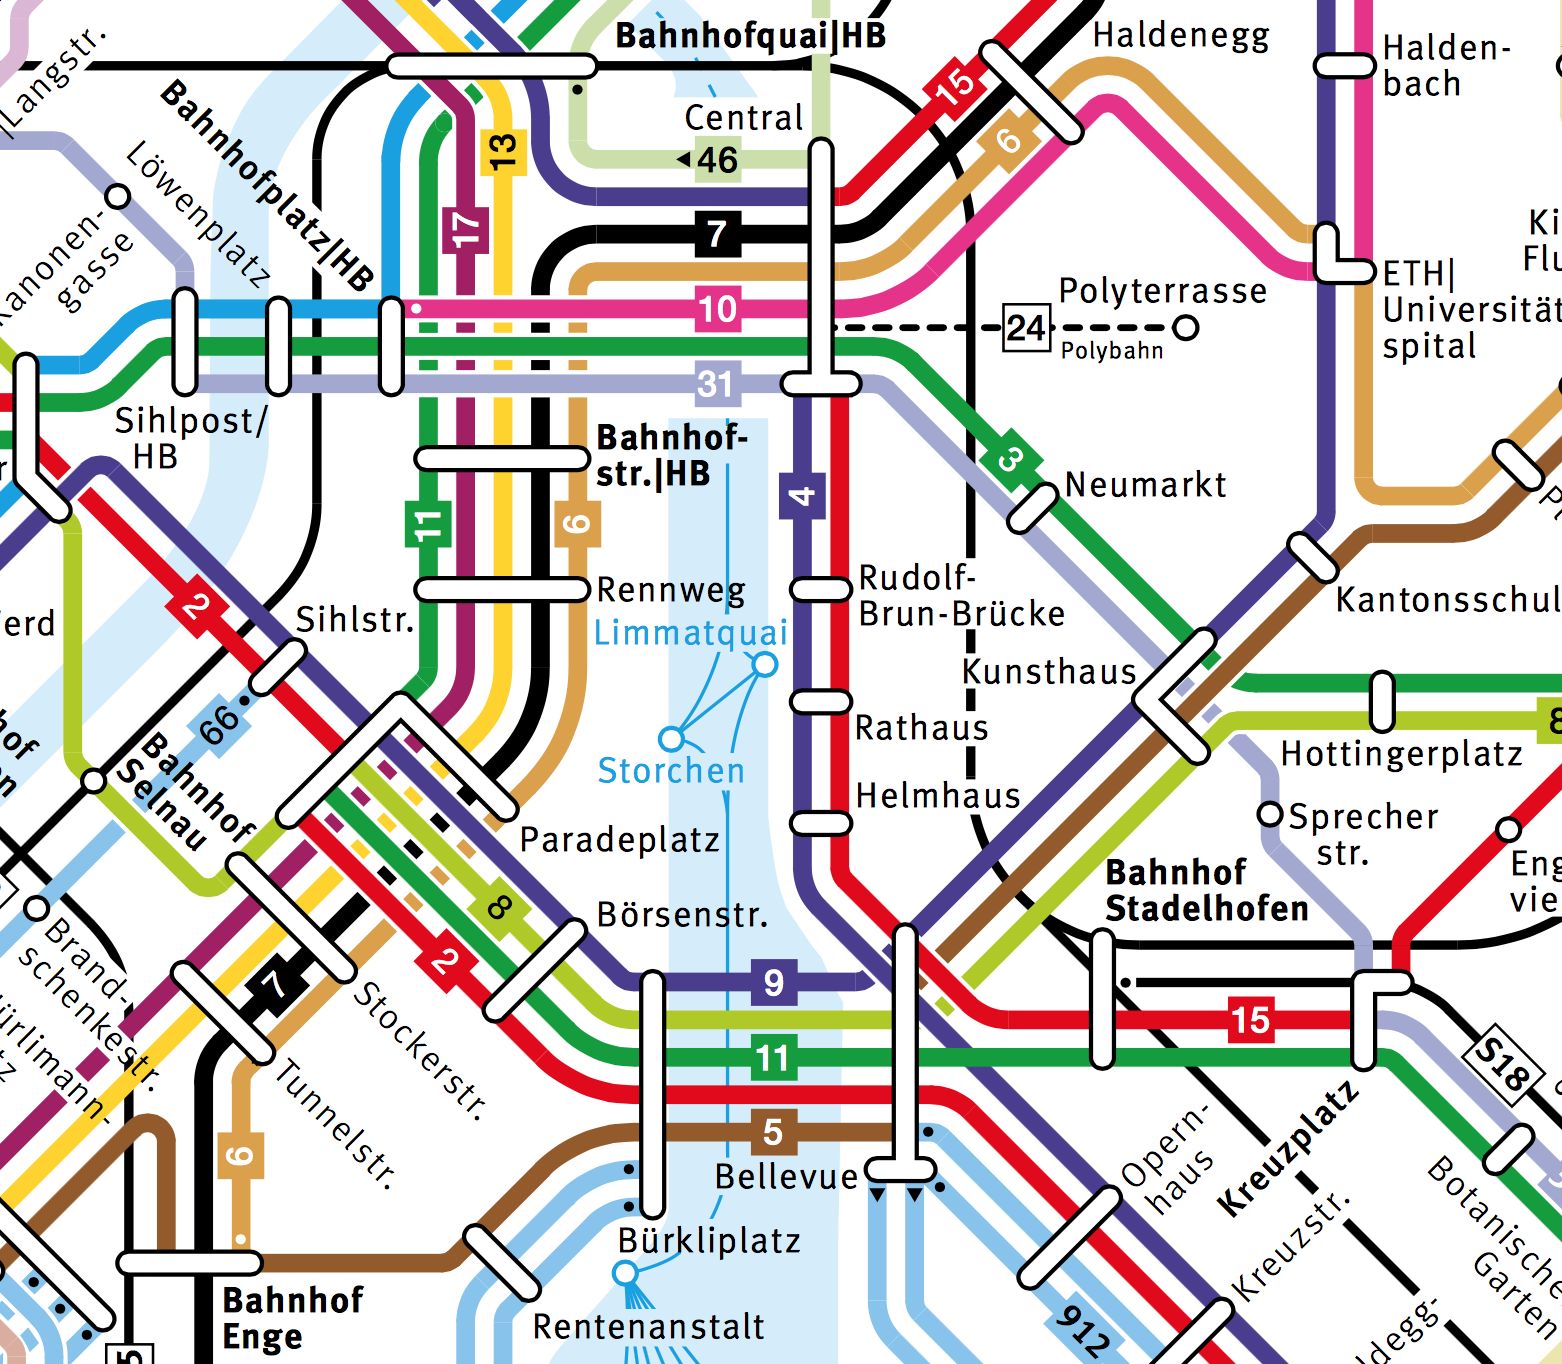
\includegraphics[width=0.97\linewidth]{../fig/zvv.png}
\caption{Ausschnitt aus dem ZVV Liniennetzplan}
\label{fig:zvv}
\end{figure}

\begin{aufg}
\"Uberlegen Sie sich, wie Sie dieses Problem mit Hilfe von einem Graphen modellieren k\"onnen und implementieren Sie den entsprechenden Graphen als Adjazenzmatrix. Betrachten Sie dabei aussschliesslich Tramlinien und -haltestellen und nur solche, die im Kartenausschnitt komplett sichtbar sind.

Handelt es sich um einen gerichteten oder ungerichteteten Graphen?
\end{aufg}

\begin{aufg}
Stellen Sie sich vor, am Bellevue werden Bauarbeiten durchgef\"uhrt und das Bellevue muss temport\"ar f\"ur den Trambetrieb geschlossen werden. Erreichen Sie von der ETH aus dennoch den Bahnhof Enge? Benutzen Sie Ihr Programm, um dies zu \"uberpr\"ufen.
\end{aufg}

\begin{aufg}
Wieviele Tramstationen m\"ussen mindestens gefahren werden, um von der ETH aus zum Bahnhof Enge zu gelangen?
\begin{enumerate}[(a)]
\item Falls das Bellevue gesperrt ist.
\item Falls das Bellevue wieder ohne Einschr\"ankungen befahrbar ist.
\end{enumerate}
\end{aufg}

\begin{aufg}
Auf welchem Weg kommen Sie am schnellsten von der ETH zum Bahnhof Enge?
\begin{enumerate}[(a)]
\item Falls das Bellevue gesperrt ist.
\item Falls das Bellevue wieder ohne Einschr\"ankungen befahrbar ist.
\end{enumerate}
\end{aufg}

\begin{aufg}
Beurteilen Sie die Laufzeit des Algorithmus in Bezug auf die Anzahl Knoten und Kanten.
\end{aufg}

\begin{aufg}
Beurteilen Sie den Speicherbedarf des Algorithmus in Bezug auf die Anzahl Knoten und Kanten.
\end{aufg}
